\documentclass{beamer}
\usepackage{geometry}
\usepackage[english]{babel}
\usepackage[utf8]{inputenc}
\usepackage{amsmath}
\usepackage{amsfonts}
\usepackage{amssymb}
\usepackage{tikz}
\usetikzlibrary{quotes, angles}
\usepackage{graphicx}
\usepackage{multicol}

%\usepackage{pgfplots}
%\pgfplotsset{width=10cm,compat=1.9}
%\usepackage{pgfplotstable}

\setlength{\headheight}{26pt}%doesn't seem to fix warning

\usepackage{fancyhdr}
\pagestyle{fancy}
\fancyhf{}

%\rhead{\small{13 September 2021}}
\lhead{\small{BECA / Dr. Huson / Geometry Unit 2}}

\renewcommand{\headrulewidth}{0pt}

\title{Mathematics Class Slides}
\subtitle{Bronx Early College Academy}
\author{Christopher J. Huson PhD}
\date{4 October 2021}

\begin{document}
\frame{\titlepage}
\section[Outline]{}
\frame{\tableofcontents}

\section{2.1 Area and volume formulas, 4 October}
\frame
{
  \frametitle{Learning Target: I can calculate area}
  \framesubtitle{7.G.B.6 Solve problems involving area, volume and surface area \hfill \alert{2.1 Monday 4 October}}
  \begin{block}{Do Now: Identify the true statements}
    \begin{multicols}{2}
    \begin{enumerate}
      \item $\angle 1 \cong \angle 2$
      \item $\angle 2 \cong \angle 4$
      \item $m\angle 1 + m\angle 4=180^\circ$
      \item $m\angle 2 + m\angle 3=90^\circ$
  \end{enumerate}
  \begin{center}
  \begin{tikzpicture}[scale=0.5, rotate=15]
    \draw [<->, thick] (0,-1.5)--(10,1.5);
    \draw [<->, thick] (2,3.5)--(7,-3.5);
    \node at (3,.4){1};
    \node at (6,-.6){3};
    \node at (5,1){2};
    \node at (4,-1){4};
  \end{tikzpicture}
  \end{center}
\end{multicols}
\end{block}
  Lesson: Test scoring, mastery; Area formulas \\[0.25cm]
  Homework: Test corrections due Friday
}

\frame
{
  \frametitle{Learning Target:  I can calculate area}
  \framesubtitle{7.G.B.6 Solve problems involving area, volume and surface area}

  \begin{block}{Copy these formulas into your notes}
    
    \begin{enumerate}
    \item Rectangle: $A=l \times w$ (Area equals length times width)
    \item Square: $A=s^2$ (Area equals side length squared)
    \item Triangle: $A=\frac{1}{2} b \times h$ (one half base times height)
    \item Trapezoid: $A=\frac{1}{2} (b_1 +b_2) h$ (Average of bases times height)
    \item Circle: $A=\pi r^2$ (pi times radius squared)
    \end{enumerate}
  \end{block}
}

\frame
{
  \frametitle{Quiz learning targets}
  \framesubtitle{1.13 Angles test October 1st}

  \begin{block}{Four mastery standards}
    \begin{itemize}
    \item Solve problems posed with positive and negative rational numbers in any form (whole numbers, fractions, and decimals). (7.EE.B.3)
        
    \item Use facts about supplementary, complementary, vertical, and adjacent angles in a multi-step problem to write and solve simple equations for an unknown angle in a figure. (7.G.B.5)
    
    \item Solve linear equations with rational number coefficients, including using the distributive property and collecting like terms. (8.EE.C.7.b)
    
    \item Use geometric shapes, their measures, and their properties to describe objects. (GEO-G.MG.1)
    \end{itemize}
  \end{block}
}

\frame
{
  \frametitle{Quiz scoring}
  \framesubtitle{1.13 Angles test October 1st}

  \begin{block}{Four mastery scores 1-4}
    \begin{enumerate}
    \item Left blank or barely attempted
    \item Many answers, often erroneous
    \item Consistently correct
    \item Uniformly correct and efficient
    \end{enumerate}
  \end{block}
}

\frame
{
  \frametitle{Quiz mastery standards}

  Mastery standards\\
    Solve problems posed with positive and negative rational numbers in any form (whole numbers, fractions, and decimals). (7.EE.B.3)\\
    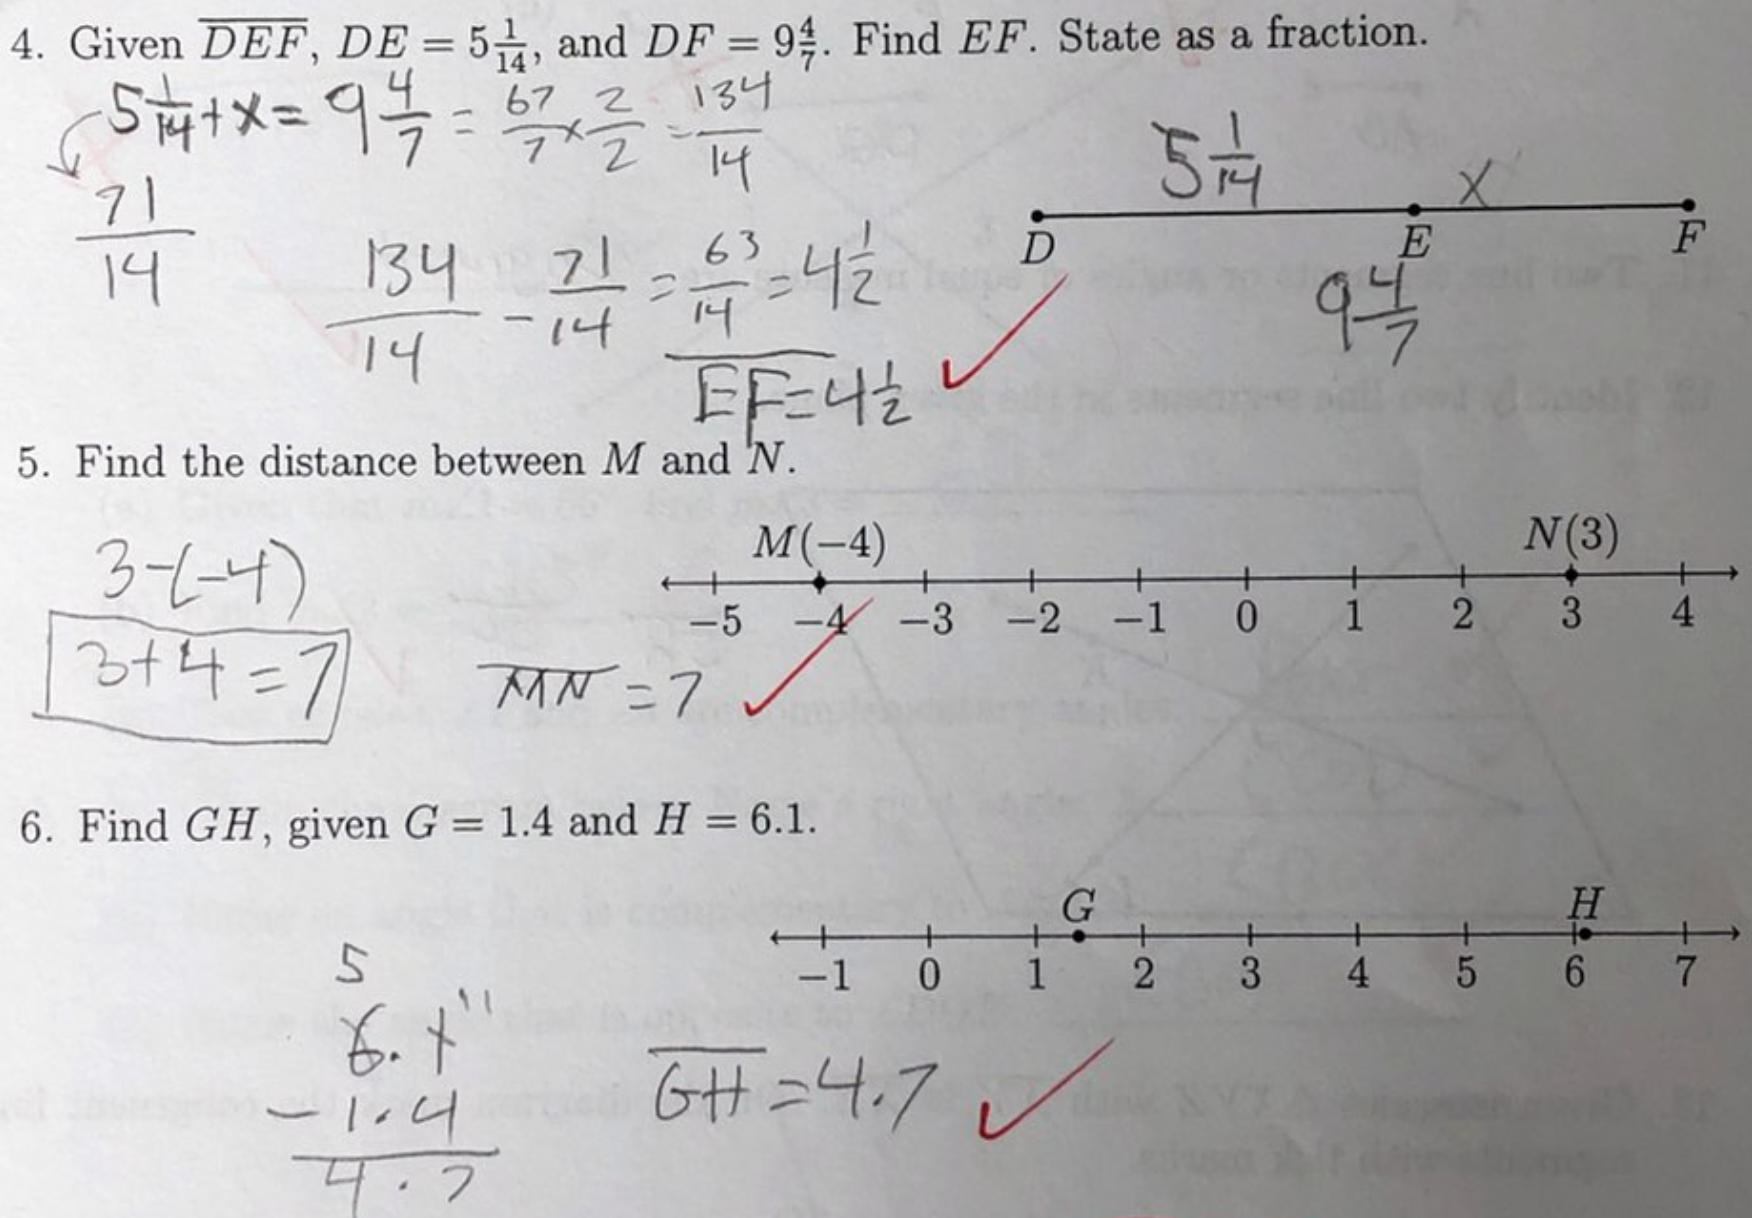
\includegraphics[width=9cm]{fractions.png}
}

\frame
{
  \frametitle{Quiz mastery standards}
  Use facts about supplementary, complementary, vertical, and adjacent angles in a multi-step problem to write and solve simple equations for an unknown angle in a figure. (7.G.B.5)\\[0.5cm]
  Solve linear equations with rational number coefficients, including using the distributive property and collecting like terms. (8.EE.C.7.b)\\
    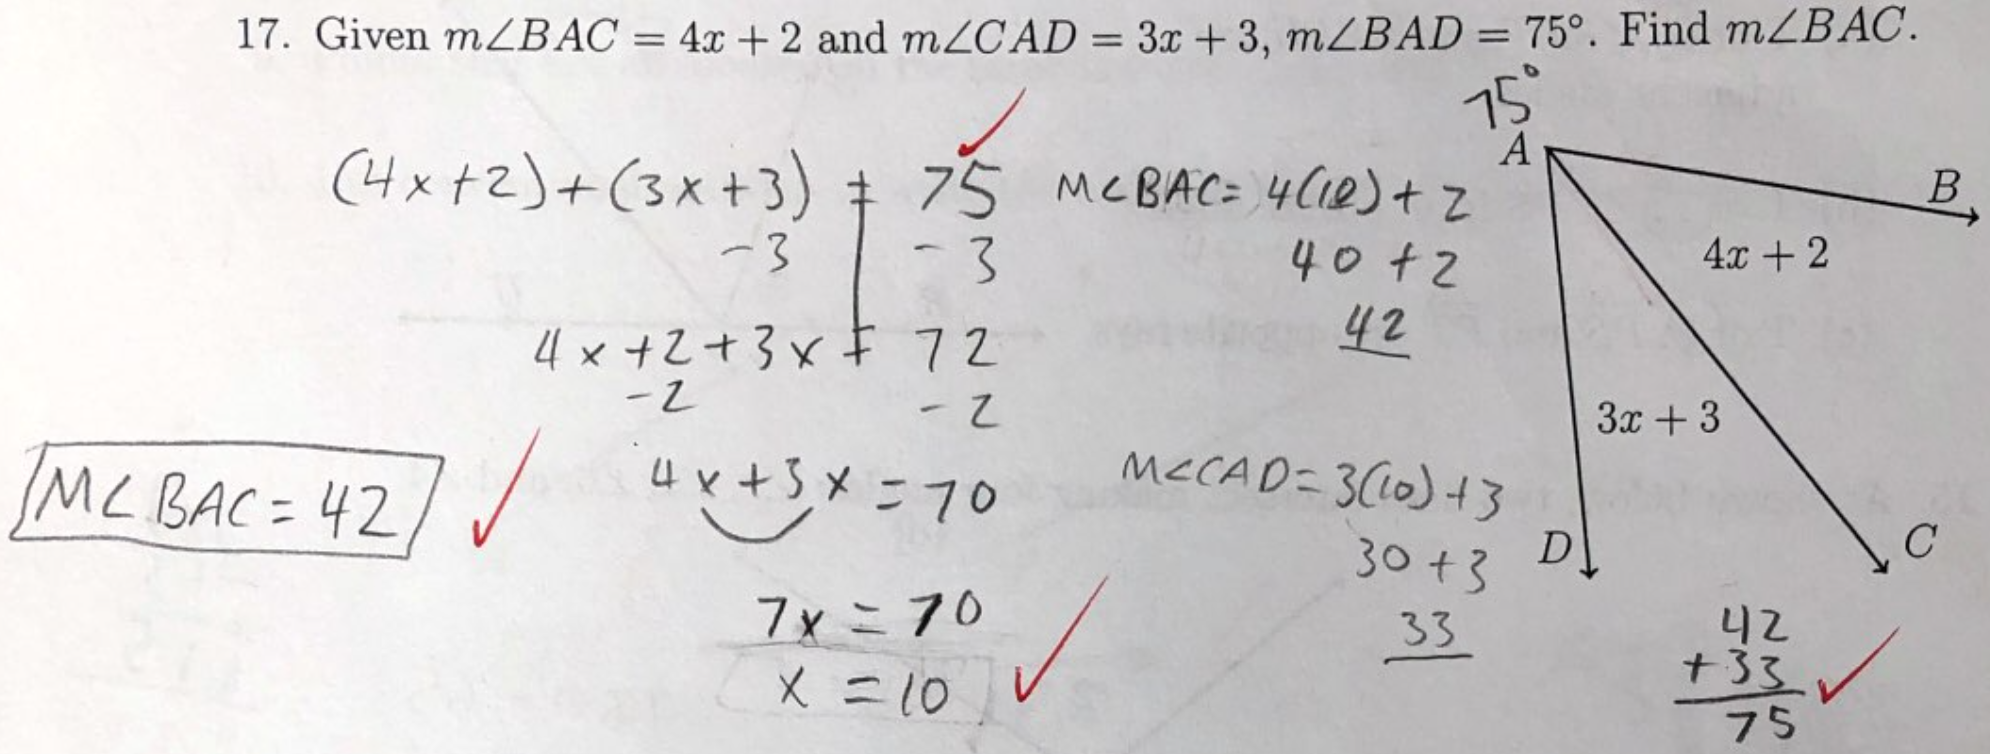
\includegraphics[width=10.5cm]{model+solve.png}
}

\frame
{
  \frametitle{Quiz mastery standards}
   Use geometric shapes, their measures, and their properties to describe objects. (GEO-G.MG.1)\\
    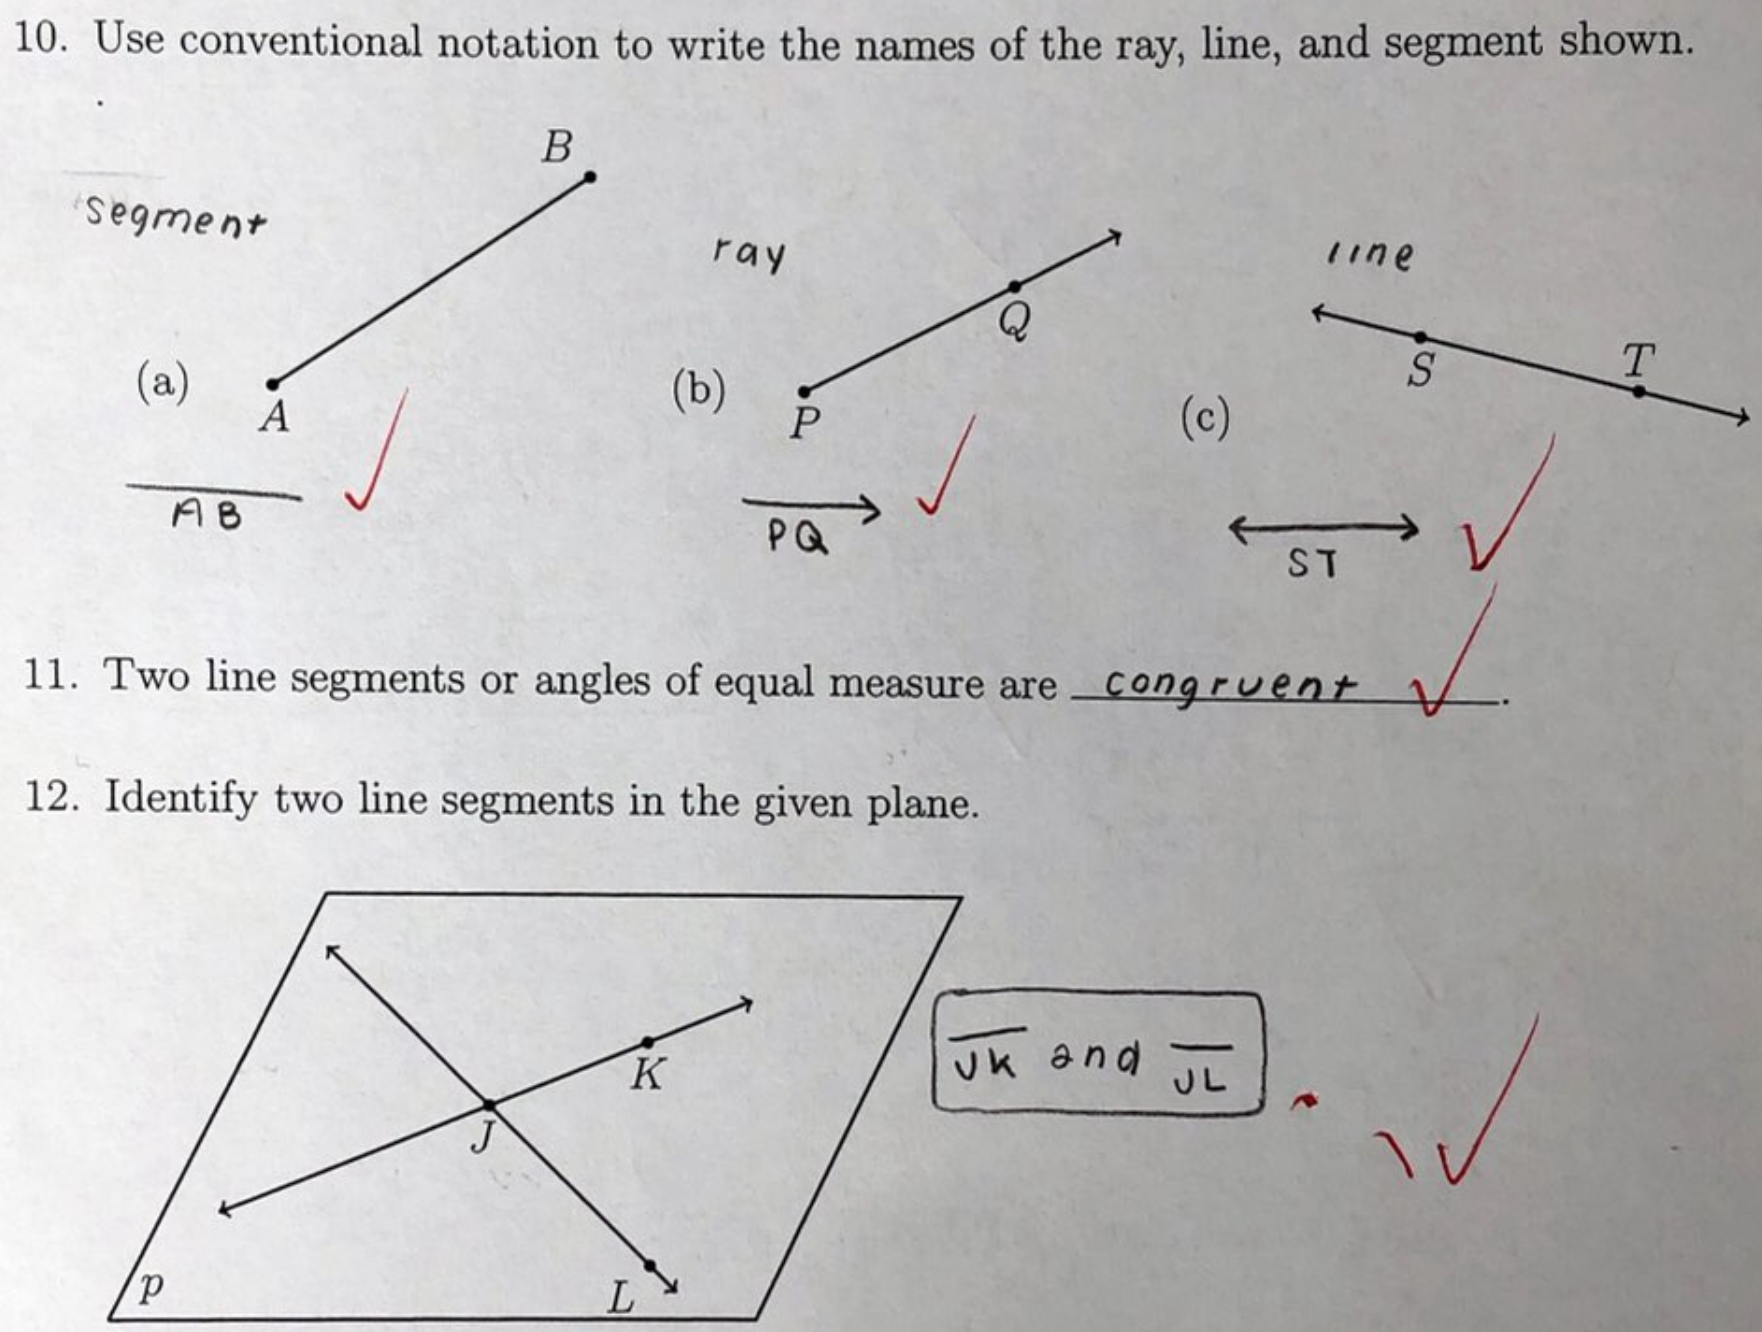
\includegraphics[width=10cm]{notationA.png}
}

\frame
{
  \frametitle{Quiz mastery standards}
   Use geometric shapes, their measures, and their properties to describe objects. (GEO-G.MG.1)\\
    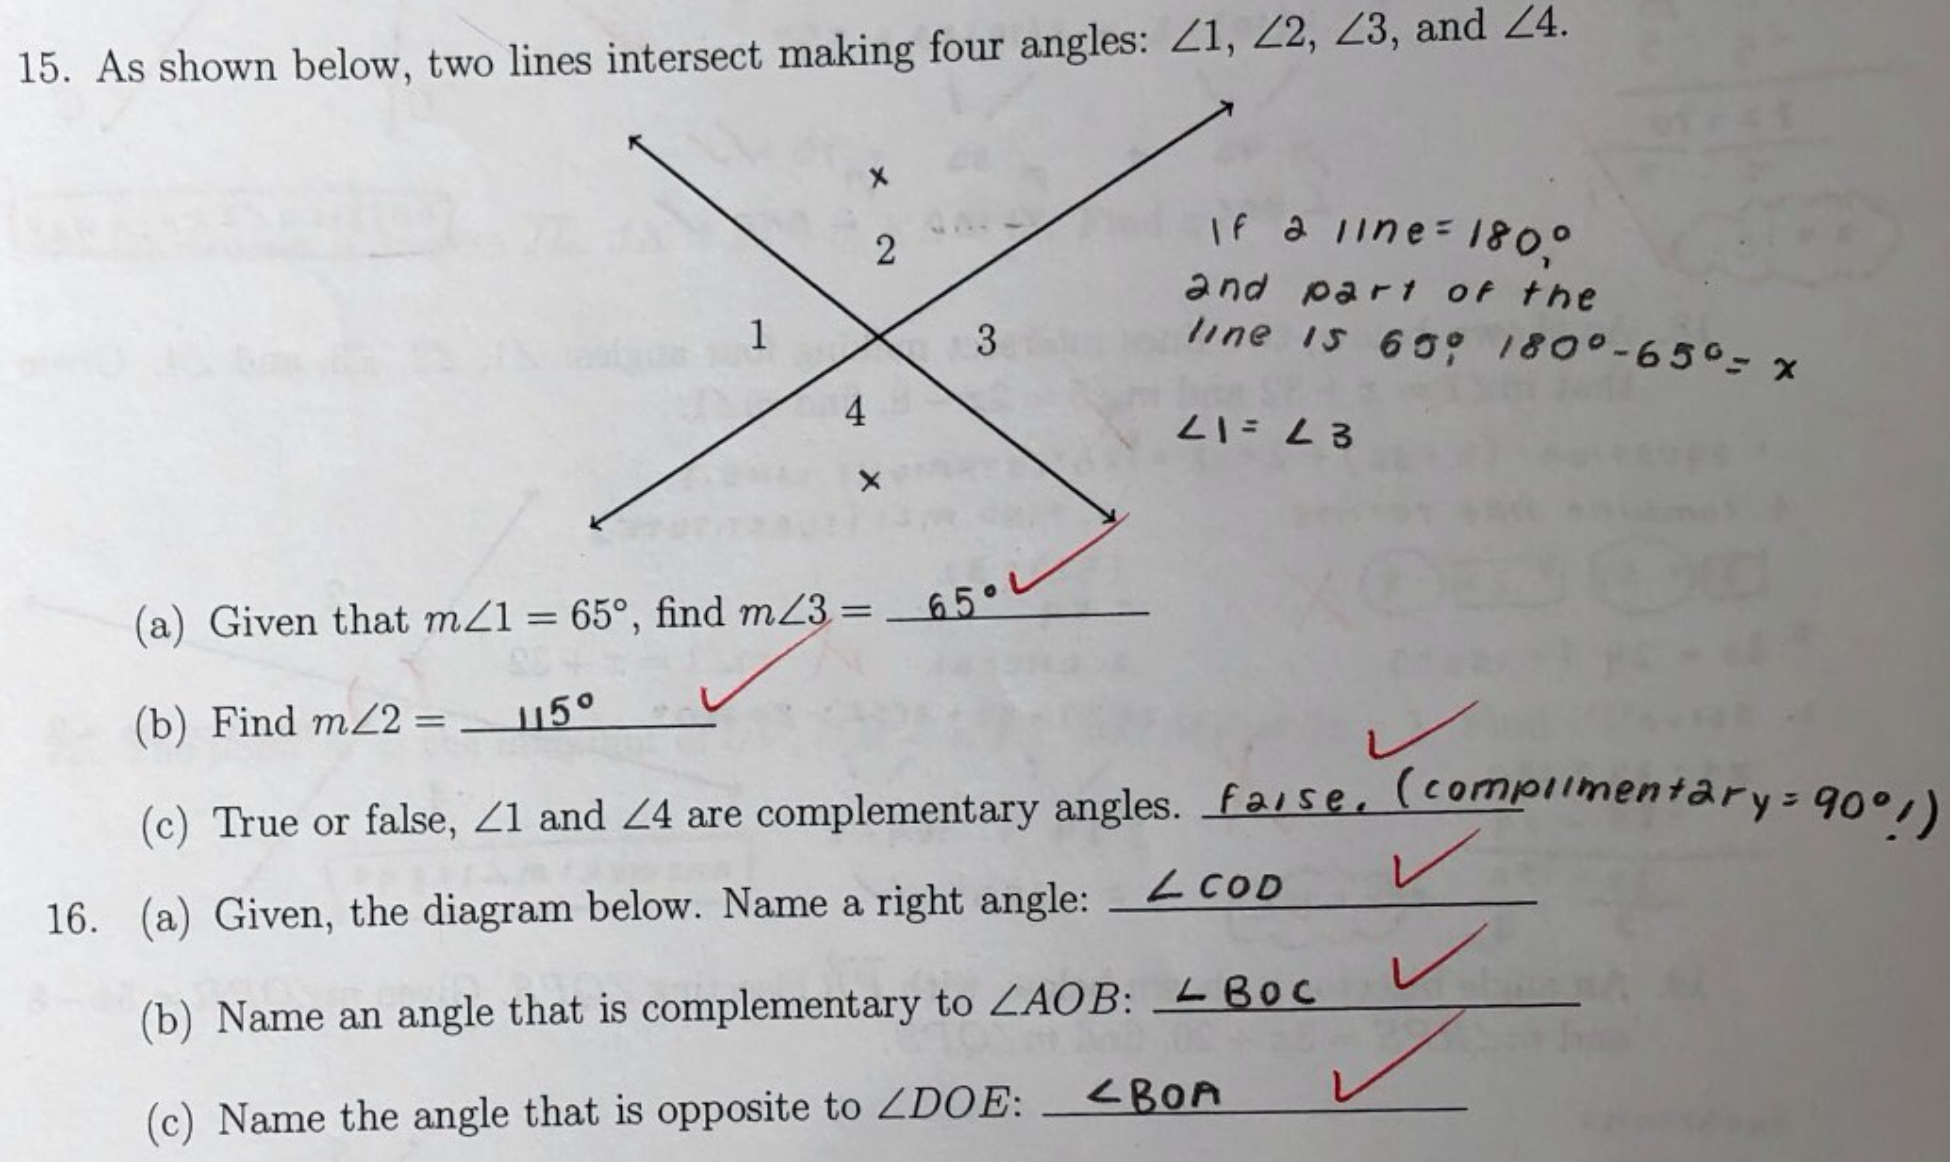
\includegraphics[width=10cm]{notationB.png}
}

\section{2.2 Area and volume formulas, 5 October}
\frame
{
  \frametitle{Learning Target: I can calculate areas}
  \framesubtitle{7.G.B.6 Solve problems involving area, volume and surface area \hfill \alert{2.2 Tuesday 5 October}}
  \begin{block}{Do Now: Identify the true statements.}
    Given $\angle AOB = 2x$ and $\angle BOC = 5x+20$.
    \begin{multicols}{2}
       \begin{enumerate}
         \item $\angle AOB \cong \angle BOC$\\
         $2x = (5x+20)$
         \item $\angle AOB$, $\angle BOC$ are complementary\\
         $2x + (5x+20)=90^\circ$
         \item $\angle AOB$ and $\angle BOC$ are a linear pair\\
         $2x + (5x+20)=180^\circ$
     \end{enumerate}
     \begin{center}
       \begin{tikzpicture}[scale=0.6, rotate=20]
         \draw [<->, thick] (-45:5)--(0,0)--(135:5);
         \draw [<->, thick] (-5,0)--(5,0);
         \draw [->, thick] (0,0)--(0,4);
         \draw (0,0)++(0.3,0)--++(0,0.3)--+(-0.3,0);
         \draw [fill] (135:3) circle [radius=0.05] node[below left]{$B$};
         \draw [fill] (-4,0) circle [radius=0.05] node[below]{$A$}; 
         \draw [fill] (0,0) circle [radius=0.05] node[below]{$O$};
         \draw [fill] (0,3) circle [radius=0.05] node[left]{$C$};
         \draw [fill] (4,0) circle [radius=0.05] node[below]{$D$};
         \draw [fill] (-45:3) circle [radius=0.05] node[above]{$E$};
         \end{tikzpicture}
     \end{center}
   \end{multicols}
   Copy the correct equation and solve for $x$. Check your answer.
\end{block}
  Lesson: Compound area situations
}

\section{2.3 Area and volume formulas, 6 October}
\frame
{
  \frametitle{Learning Target: I can calculate areas}
  \framesubtitle{7.G.B.6 Solve problems involving area, volume and surface area \hfill \alert{2.3 Wednesday 6 October}}
  \begin{block}{Do Now: Identify the true statements.}
    Ray $\overrightarrow{KM}$ bisects $\angle JKL$. $m\angle JKM = 4x-20$, $m\angle MKL = 3x+4$.
    \begin{multicols}{2}
      \begin{enumerate}
        \item $\angle JKM$ and $\angle MKL$ are a linear pair\\
        $(4x-20) + (3x+4)=180^\circ$
        \item $\angle JKM$, $\angle MKL$ are adjacent and\\
        $4x-20 =90^\circ$
        \item $\angle JKM \cong \angle MKL$\\
        $4x-20 = 3x+4$
    \end{enumerate}
    \begin{center}
      \begin{tikzpicture}[scale=0.5, rotate=-10]
        \draw [<->, thick] (160:5)node[below left]{$J$} 
        --(0,0)node[below left]{$K$}
        --(10:5)node[above right]{$L$};
        \draw [->, thick] (0,0)--(90:5)node[below left]{$M$};
        %\draw [fill] (0,0) circle [radius=0.05] node[below]{$A$};
        %\draw [fill] (5,0) circle [radius=0.05] node[below]{$B$};
      \end{tikzpicture}
    \end{center}
  \end{multicols}
   Copy the correct equation and solve for $x$. Check your answer.
\end{block}
  Lesson: Compound area situations
} 

\section{2.4 Perimeter, 7 October}
\frame
{
  \frametitle{Learning Target: I can calculate areas}
  \framesubtitle{7.G.B.6 Solve problems involving area, volume and surface area \hfill \alert{2.4 Thursday 7 October}}
  \begin{block}{Do Now: Find the area of the shape with lengths marked}
    All angles are $90^\circ$. (not drawn to scale)
    \begin{flushleft}
    \begin{tikzpicture}[scale=0.8]
      \draw [-, thick] (0,0)--(5,0)--(5,2)--(3,2)--(3,3)--(0,3)--cycle;
      \node at (5.5, 1){5};
      \node at (1.5, 3.5){7};
      \node at (2.5, -0.5){12};
      \node at (-0.5, 1.5){7};
    \end{tikzpicture}
    \end{flushleft}
\end{block}
  Lesson: Perimeter\\
  Exit quiz: Use angle facts to write equations, solve linear equations
} 

\section{2.5 Volume formulas, 8 October}
\frame
{
  \frametitle{Learning Target: I can calculate volume}
  \framesubtitle{7.G.B.6 Solve problems involving area, volume and surface area \hfill \alert{2.5 Friday 7 October}}
  \begin{block}{Do Now: Find the area and perimeter of the shape}
    Angles that appear to be square are $90^\circ$. (not drawn to scale)
    \begin{flushleft}
    \begin{tikzpicture}[scale=0.8]
      \draw [-, thick] (0,0)--(5,0)--(3,1.5)--(3,1.5)--(3,3)--(0,3)--cycle;
      \draw [-, dashed] (3,0)--(3,1.5);
      \node at (3.3, 2.2){3};
      \node at (4, 1.1){5};
      \node at (1.5, 3.5){5};
      \node at (2.5, -0.5){9};
      \node at (-0.5, 1.5){6};
    \end{tikzpicture}
    \end{flushleft}
\end{block}
  Lesson: Volume\\
  Review yesterday's quiz: Use angle facts to write equations, solve linear equations
} 

\frame
{
  \frametitle{Learning Target:  I can calculate volume}
  \framesubtitle{7.G.B.6 Solve problems involving area, volume and surface area}

  \begin{block}{Copy these formulas into your notes}
    
    \begin{enumerate}
    \item Rectangular prism (box): $V=l \times w \times h$ \\(Volume equals length times width times height)
    \item Cube: $V=s^3$ (Area equals side length cubed)
    \item Pyramid: $V=\frac{1}{3} B \times h$ (where $B$ is the area of the base)
    \item Cone: $V=\frac{1}{3} (\pi r^2) h$ 
    \item Sphere: $V=\frac{4}{3}\pi r^3$
    \end{enumerate}
  \end{block}
}

  \frame
  {
    \frametitle{Casio fx-9750GII calculator - due Friday 1 October}
    \begin{multicols}{2}
    In the high school at BECA we use the Casio fx-9750GII.\\[5pt] 
    It is allowed on the Regents exams, SAT tests, and International Baccalaureate exams.\\[5pt]
    You may use a different calculator in Geometry if you prefer, but I recommend buying the Casio fx-9750GII.\\[5pt]
    (see me if buying a calculator is a hardship for your family)
    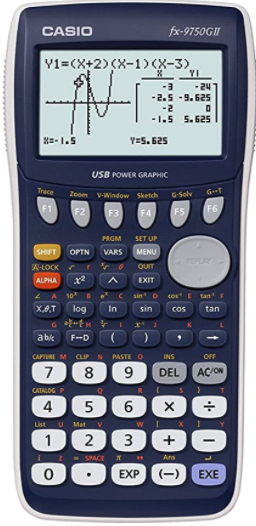
\includegraphics[width=3.5cm]{casio_fx-9750GII.png}
    \end{multicols}
  }

  \frame
  {
    \frametitle{Learning Target: I can use technology}
    \framesubtitle{CCSS: MP4 use technology strategically}
  
    \begin{block}{Self assessment: Technology}
      
      \begin{enumerate}
      \item I have my own calculator with me today. Yes \qquad No
      \item I have a notebook, ruler, and protractor. Yes \qquad No
      \end{enumerate}
    \end{block}
  }

  \frame
  {
    \frametitle{Open Middle problem (fun) \\
    Use digits from 0 to 9. Using a digit no more than once.}
      The first two angle measures are complementary. The second two angles supplementary. (degrees)\\[0.75cm]
        \begin{tikzpicture}
          \draw (0,0) rectangle (1,1);
          \draw (1.25,0) rectangle (2.25,1);
          \draw (3.25,0) rectangle (4.25,1);
          \draw (4.5,0) rectangle (5.5,1);

          \draw (-1.25,-1.5) rectangle (-0.25,-0.5);
          \draw (0,-1.5) rectangle (1,-0.5);
          \draw (1.25,-1.5) rectangle (2.25,-0.5);
          \draw (3.25,-1.5) rectangle (4.25,-0.5);
          \draw (4.5,-1.5) rectangle (5.5,-0.5);
        \end{tikzpicture} \vspace{5cm} 
  }

  \section{414 Seating chart 10.1}
  \frame
  {
    \frametitle{414 Seating chart 10.1}
    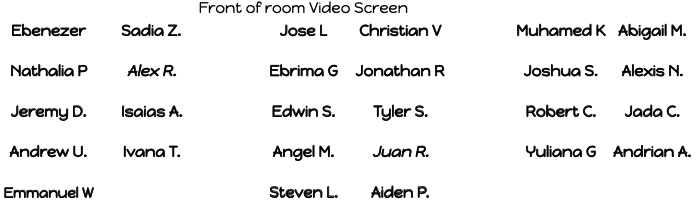
\includegraphics[width=11cm]{Seating_10A-414.png}
  }

  \section{420 Seating chart 10.3}
  \frame
  {
    \frametitle{420 Seating chart 10.3}
    \begin{center}
      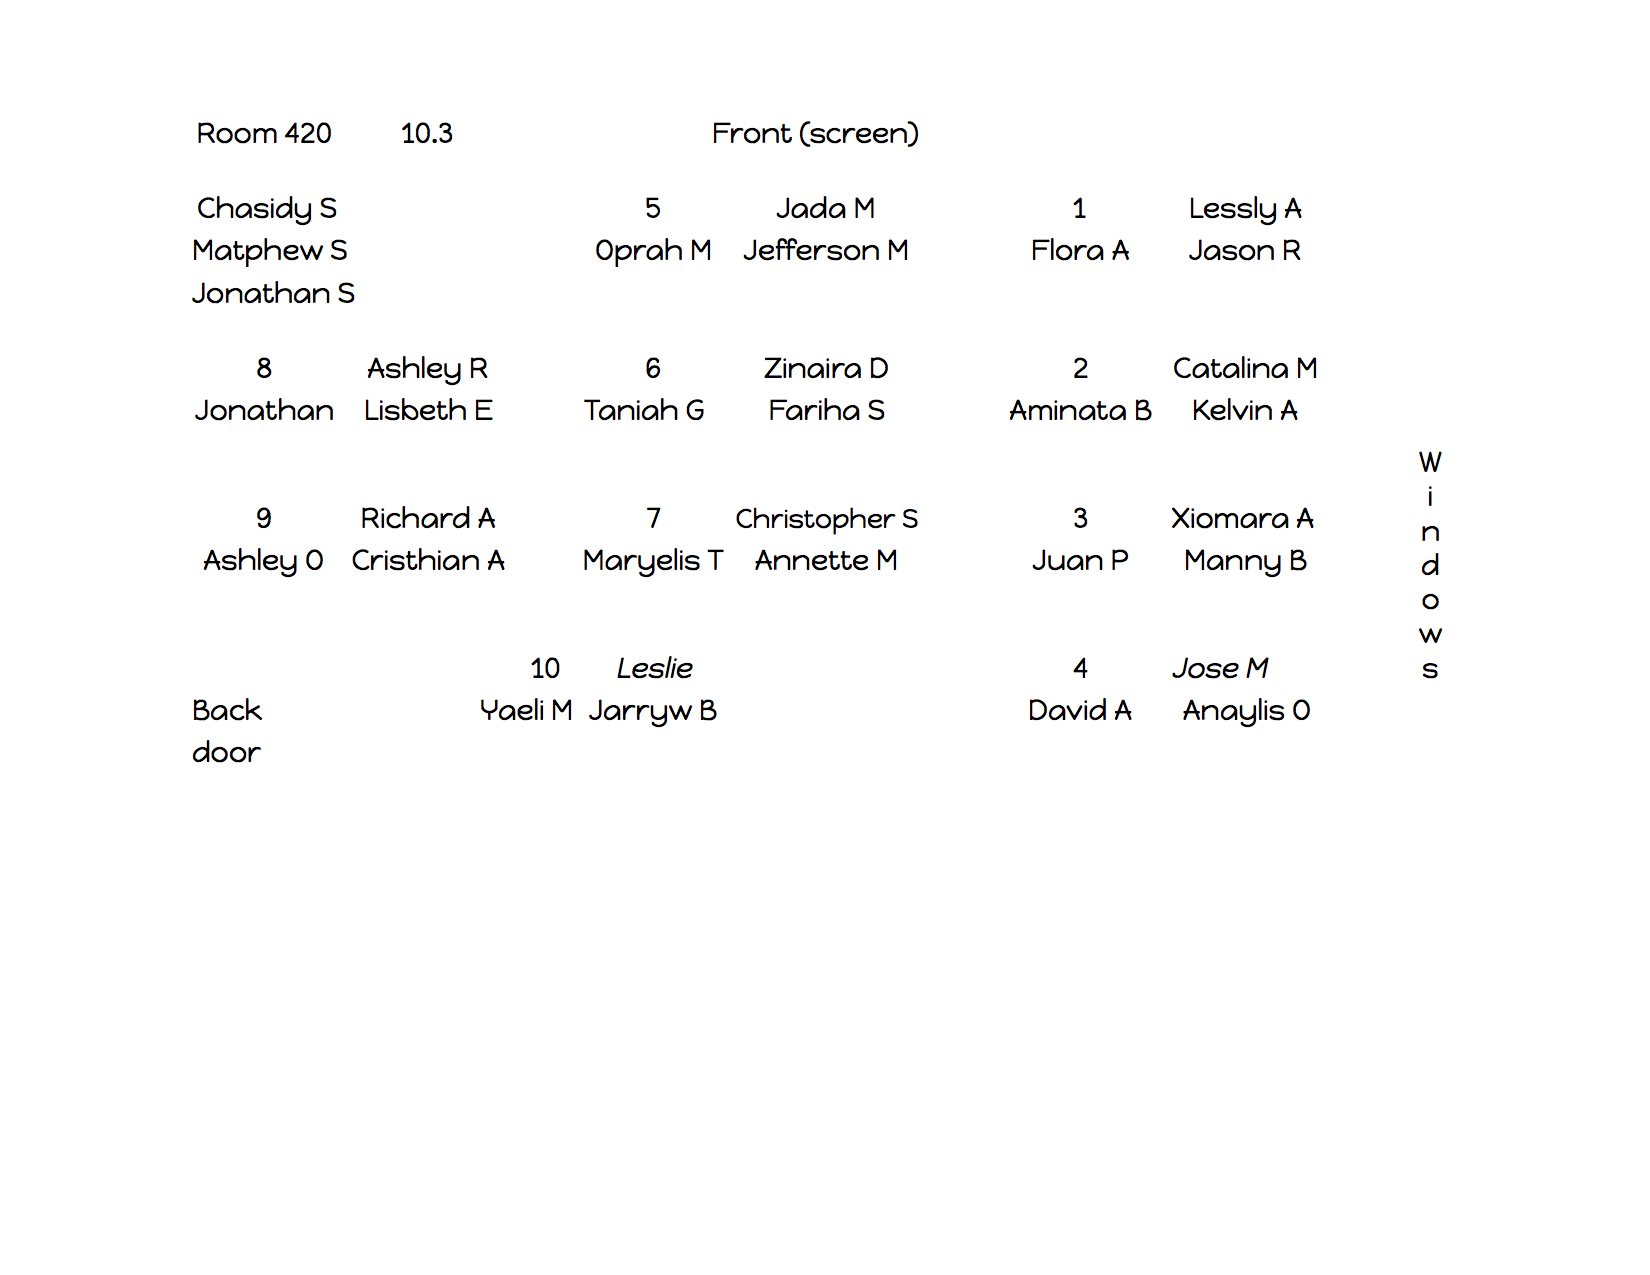
\includegraphics[width=11cm]{10C_seating.png}
    \end{center}
  }

\frame
{
  \frametitle{Quiz learning targets}
  \framesubtitle{7.G.B.6 Solve problems involving area, volume and surface area}

  \begin{block}{Four mastery standards}
    \begin{itemize}
    \item Solve multi-step real-life and mathematical problems posed with positive and negative rational numbers in any form (whole numbers, fractions, and decimals), using tools strategically. Apply properties of operations to calculate with numbers in any form; convert between forms as appropriate; and assess the reasonableness of answers using mental computation and estimation strategies. For example: If a woman making \$25 an hour gets a 10\% raise, she will make an additional 1/10 of her salary an hour, or \$2.50, for a new salary of \$27.50. If you want to place a towel bar 9 3/4 inches long in the center of a door that is 27 1/2 inches wide, you will need to place the bar about 9 inches from each edge; this estimate can be used as a check on the exact computation. (7.EE.B.3)
        
    \item Use facts about supplementary, complementary, vertical, and adjacent angles in a multi-step problem to write and solve simple equations for an unknown angle in a figure. (7.G.B.5)
    
    \item Solve linear equations with rational number coefficients, including equations whose solutions require expanding expressions using the distributive property and collecting like terms. (8.EE.C.7.b)
    
    \item Use geometric shapes, their measures, and their properties to describe objects. (GEO-G.MG.1)
    \end{itemize}
  \end{block}
}
  


\end{document}